% !TEX root = ../thesis-sample.tex

\chapter{Autonomous Exploration in Vertically-Uniform 3D Space} \label{chap:ae3Dsimple}

In this chapter, we introduce mapping and autonomous exploration in 3D environments. Here, we consider common spaces like rooms and hallways where objects are largely vertically-uniform. A complete 3D probabilistic map is projected onto a simpler 2D map at a fixed exploration height, where the projected map can be used for collision-avoidance and entropy predictions.

\section{Occupancy Grid Mapping in 3D}

The inverse sensor model from Chapter \ref{chap:pogm} is based on an arbitrary vector spanning 2D space. The distances from the robot to grid cells are obtained geometrically through ray casting. This method is easily extended to 3D space, and the inverse sensor model is applied identically. Since the map is updated ray-by-ray (each measurement ray is considered once by itself), this approach is extended for measurement fusion of any number of sensors; the map is updated by each ray of a scan sequentially, then the map is updated by the rays of the next scan in queue, which might have different characteristics. There are several reasons why a robot might be equipped with multiple sensors, e.g., different fields-of-view or depth sensor properties. For example, a robot may be equipped with a 2D LIDAR with highly accurate measurements, but a limited single-plane field-of-view. Then, the robot can compensate for the LIDAR limitations with an IR depth sensor that provides many more measurement rays with a 3D scan, where each ray has lower accuracy than the LIDAR rays. Since each sensor model is explicitly considered in the cell probability calculations, measurements from both sensors may serve to update the same probabilistic map. However, the impact from a LIDAR measurement with high accuracy on the probabilistic map will be greater than that of the IR depth sensor with lower accuracy. Since sensor properties are considered explicitly, the proposed 3D mapping approach can fuse the impact of measurements on the probabilistic map from different sources with different properties.

However, implementation in 3D requires several careful considerations. First, the number of cell occupancy probabilities tracked with computer memory increases by a factor of the number of cells in the added dimension. In its current form, the proposed method assumes fixed map limits, so these should be carefully selected with grid cell resolution based on available memory. Second, measurement rays spanning 3D space typically involve more intersections with grid cells. The computational orders of ray casting and the inverse sensor model are proportional to the number of grid cells along the ray $n_r$, so careful consideration must be placed on sensor limits and rays per scan that can be considered. Typically, computers small enough to be carried onboard flying robots lack the processing capabilities to update massive maps quickly, particularly because the ray-by-ray updating method requires many computations in series with large measurement scans. Therefore, an onboard computer can simply stream the sensor data, and a more powerful computer can run the mapping.

Additionally, mobile robots, particularly aerial vehicles, are frequently subject to fast movements, and the time stamps for pose estimates and depth sensor readings are not guaranteed to align. For example, the most recent pose estimate and measurement scan may have significantly different time stamps while the robot is rapidly rotating. Using these together violates the assumption that the robot pose is well-known for every measurement scan, i.e., $X_t$ and $Z_t$ are given. Therefore, pose estimates and sensor readings must be paired according to their time stamps. A useful tool that easily satisfies this goal is the Message Filters package with the Robot Operating System (ROS), where stamped poses and measurement scans are synchronized using recently-received data.

\section{Exploration in Vertically-Uniform Environments}
\label{sec:MapProjections}

Next, we describe two approaches to projecting the 3D probabilistic map onto a 2D map at the exploration height. Assuming projections are sufficient is consistent with rooms and hallways with non-complex geometries.

\subsubsection{Collision and Entropy Maps}
Occupancy grid map cell volume is frequently smaller than the size of the robot taking measurements, particularly with highly-detailed maps. This motivates a method to simply represent locations that risk collision, referred to as a \emph{collision map} $C$. Let $k_C\geq1$ be an integer representing the minimum number of 3D grid cells that form a cube that can completely encompass the robot, i.e., the collision map cell edge length is
\begin{align}
\label{eqn:alphaC}
\alpha_C=k_C\alpha.
\end{align}
Consider the set $ m_{C,k}\subset m$ consisting of the 3D grid cells falling inside the limits of the $k$-th cell of collision map $C$, namely $\mathbf{C}_k$. Then the collision probability is
\begin{align}
P(\mathbf{C}_k)=\max{(P(\mathbf{m}_i)\ \forall \ i\in m_{C,k})}.
\end{align}
Then, the robot is only allowed to consider moving into $k$-th cell of the collision map if
\begin{align}
P(\mathbf{C}_k) \leq C_\text{thresh},
\end{align}
where $C_\text{thresh}>0$ is a maximum acceptable collision threshold, typically chosen slightly greater than $0$. In short, this conservative approach limits robotic motion to regions with a low risk of collision while neglecting objects far above or below the exploration plane.

In a similar method, \emph{entropy map} $E$ determines cells based on the entropy metric of \refeqn{ShannonsEntropyCell} over a different subset of cells. Let the $E$ be a 2D map composed of cells with edge length $\alpha$ located at the exploration height. Let the set $ m_{E,k}\subset m$ be the cells directly above and below the $k$-th cell of $E$, neglecting any 3D cells located lower than the floor height. Selecting this set is advantageous because measurements are assumed not to penetrate occupied cells (edge length $\alpha$) and measurement rays are typically not closely-aligned with the third axis of the inertial frame (vertically long set). Furthermore, any cells located below the floor, which cannot be reached, should not impact the uncertainty of the space. Then, the occupancy probability of the $k$-th entropy map cell is selected as
\begin{align}
\label{eqn:ProbEntropyMap}
P(\mathbf{E}_k)=\argmax_{P(\mathbf{m}_i)}(H(P(\mathbf{m}_i))\ \forall \ i\in m_{E,k}).
\end{align}
After several measurements of the cells belonging to $ m_{E,k}$, it is common for $H(P(\mathbf{E}_k))\approx0$, which implies that these cells are well-known. However, this does not imply that the captured space is \emph{entirely} free or occupied (e.g. an object on the ground that does not breach the upper map boundary), so applying \refeqn{ProbEntropyMap} alone could arbitrarily set $P(\mathbf{E}_k)$ close to $0$ or $1$. This can have damaging effects on the expected information of cells beyond the $k$-th cell. Let $P_\text{min}>0$ be a lower bound such that $H(P_\text{min})=H(1-P_\text{min})\approx0$. If $H(P(\mathbf{E}_k))\leq H(P_\text{min})$, then this probability is corrected to
\begin{align}
P(\mathbf{E}_k)= 
\begin{cases}
    P_\text{min},			& \text{if } \text{mean}(P(\mathbf{m}_i)\ \forall \ i\in m_{E,k})\leq0.5\\
    1-P_\text{min},              & \text{otherwise}
\end{cases},
\end{align}
where the first case corresponds to mostly open space and the second case corresponds to mostly occupied space (e.g. walls and objects). In short, the candidates are only considered if they can be reached over collision map $C$ via Dijkstra's search, and the information gains of the reachable candidates are predicted using entropy map $E$.

\subsubsection{Collision and Entropy Combination Map}
The second proposed technique combines the advantages of both the collision and entropy maps into a 2D projected occupancy grid map, which can be used for both tasks. Let the \emph{collision and entropy combination map} $ m_\text{2D}$ be a 2D projected map located at the exploration height with grid cell edges the same as the collision map, namely $\alpha_C$ from \refeqn{alphaC}, using the same subset of grid cells from the collision map, namely $ m_C$. Considering that the cells begin with uniform probability $P_\text{init}$ where $0<P_\text{init}<1$, define a threshold $P_\text{thresh}$ such that $P_\text{init}<P_\text{thresh}<1$. Then, the probability assigned to the $k$-th grid cell of $ m_\text{2D}$, namely $\mathbf{m}_{\text{2D},k}$ is
\begin{align}
\label{eqn:CombinationProjection2DMap}
P(\mathbf{m}_{\text{2D},k})= 
\begin{cases}
    P(\mathbf{C}_k),			& \text{if }P(\mathbf{C}_k)\geq P_\text{thresh}\\
    \min{(P(\mathbf{m}_i)\ \forall \ i\in m_{C,k})},              & \text{otherwise}
\end{cases}.
\end{align}

This approach has several advantages. First, measurements must enter the vicinity of the $k$-th cell for $P(\mathbf{m}_{\text{2D},k})$ to change from $P_\text{init}$. Without prior measurements, capturing $P(\mathbf{m}_{\text{2D},k})$ produces a large reward for the expected information gain in \refeqn{ObjFun}. Second, the value of $P_\text{thresh}$ can be modified based on how conservative the collision risk assessment for a robot should be. Additionally, when $P(\mathbf{m}_{\text{2D},k})<P_\text{thresh}$, this event tends to favor free cells such that expected information gains of cells beyond the $k$-th cell have greater impact on exploration. Furthermore, a single map is simpler, and since cell sizes satisfy $\alpha_C\geq\alpha$, it follows that $n_r$ can only be decreased with $\alpha_C$, thereby increasing computational speed.

\section{Numerical Example}
\label{sec:Compare2MapProjections}

The following numerical example involves a simulated quadrotor taking measurements of a large room and generating a 3D occupancy grid map. Separate collision and entropy map projections are used for autonomous exploration.

\subsection{Software Structure}
%        A.      Software Structures
%                list and explain ROS nodes

The Robot Operating System (ROS) provides an excellent framework for several programs, referred to as \emph{nodes}, to communicate easily. These are mostly coded in C++ for speed, except for a few Python scripts for a GUI and trivial message conversions, and launch/yaml scripts for running nodes and setting parameters. 

Gazebo is a 3D dynamic simulator~\cite{KaeHow04}, with plugins to simulate an Asus Xtion color depth sensor and a Hokuyo LIDAR. Gazebo also provides position and attitude transforms from the world to the quadrotor body, and the ability to set robot model states directly. 

Using fixed transformations between the quadrotor body and its onboard sensors, an original mapping node uses a variation of ROS message filters, known as transform message filters, to synchronize the sensor poses with sensor readings. These serve as inputs for ray casting in 3D, which provides the cell probabilities and depths along the ray through geometry. Then, the inverse sensor model serves to update the map ray-by-ray.  The node is designed to work for any number of sensors, specified by sensor parameters in a yaml configuration file.

There are two processes for exploration. The first process is projecting the 3D map onto 2D maps; the same code under different conditional parameters produces two nodes, for collision and entropy maps. The second process subscribes to these two 2D maps; the collision map serves as input for candidate pose consideration and Dijkstra's search, and the entropy map serves to predict information gain. This node provides path messages, composed of desired poses $0.01$ sec apart, displayed with a ROS visualization package, Rviz.

Finally, a path-interpreter node subscribes to the path messages and interpolates the pose at the current ROS time step. This pose is converted into a message that sets the Gazebo quadrotor state.



\subsection{Simulation Results}
%        B.      Simulation Results
%                a little bit more interpretations for the results


The 3D mapping and exploration algorithms are simulated with several parameters, described next.

\paragraph{Maps}

A cell size of $\alpha=0.075$ m is selected and the map limits are $-4$ m to $4$ m in the x-direction, $-6$ m to $6$ m in the y-direction, and $-0.15$ m to $1.5$ m in the z-direction. The initial probability of cells is selected at $P_\text{init}=0.1$. For the collision map, the cell edge factor is $k_C=3$. Additionally, Dijkstra's algorithm produces a cost map composed of distance costs for each collision map cell, denoted $d_\text{cell}$, from the current robot position to the candidate pose locations over a collision-free path about the occupancy grid. 

\paragraph{Sensors}

Next we describe the key parameters used for mapping and exploration. The inverse sensor model \refeqn{RayISMAnswer}--\refeqn{Unnormalized} relies on the stochastic properties of two sensors, namely an Asus Xtion color IR depth sensor and a Hokuyo LIDAR. The Xtion and Hokuyo sensors are modeled using a modified version of the beam model for range finders~\cite{ThrBurFox05}. This includes uniform distribution for a phantom reading with probability $P_\text{rand}=0.1$ and a Gaussian distribution with probability $P_\text{hit}=0.9$. The Gaussian distribution corresponds to the desired case when the measurement $z$ correctly captures a particular cell at expected distance $\hat{z}$ with standard deviation $\sigma$. The total forward sensor model for the Xtion and Hokuyo is
\begin{align}
%p_\text{total}(z,z_\text{min},z_\text{max},\hat{z},\sigma)&=P_\text{rand}p_\text{rand}(z,z_\text{min},z_\text{max})+P_\text{hit}p_\text{hit}(z,\hat{z},\sigma),
&p_\text{total}=P_\text{rand}p_\text{rand}+P_\text{hit}p_\text{hit},
\\
&p_\text{rand}(z,z_\text{min},z_\text{max})=\frac1{z_\text{max}-z_\text{min}},
\\
&p_\text{hit}(z,\hat{z},\sigma)=\frac1{\sqrt{2\pi\sigma^2}}\exp\braces{\frac{(\hat{z}-z)^2}{{2\sigma^2}}},
\end{align}
such that $z_\text{min}=0.5$ m and $z_\text{max}=4.0$ m for both the Xtion and Hokuyo, and the standard deviations are $\sigma_\text{Xtion}=0.25$ m and $\sigma_\text{Hokuyo}=0.1$ m, respectively, which exceed their specified values to account for localization uncertainty and sensor distortion of the Xtion. These sensors update the probabilities of cubic 3D cells with edge length $\alpha=0.075$ m and initial probability $P_\text{init}=0.1$.

\paragraph{Bump Function}
Dijkstra's algorithm produces a cost map composed of distance costs for each collision map cell, denoted $d_\text{cell}$, from the current robot position to the candidate pose locations over a collision-free path about the occupancy grid. This cost map provides a more accurate travel distance cost than the Euclidean distance used in \refeqn{ObjFunApproxCompleteCartesian} because the cost map can account for obstacles within the environment, which is particularly important to properly analyze long trajectories. Therefore, we replace $k_\text{dist}\norm{x_t-x_c}^2$ from \refeqn{ObjFunApproxCompleteCartesian} with a normalized variation on the \emph{bump function}~\cite{Joh06} with maximum distance $d_\text{max}>0$,
\begin{align}
\label{eqn:BumpFunRef}
\text{bump}(d)= 
\begin{cases}
    \exp\braces{{1-\frac1{1-(d/d_\text{max})^2}}},			& \text{if }0<d<d_\text{max}\\
    0,              				& \text{otherwise}
\end{cases},
\end{align}
such that $d_\text{max}$ is selected as the maximum cost map value. Then, $\text{bump}(d)$ is multiplied to $\sum_{z_{c,i}\in R_{c}^*\text{ FOV}}\bigg(H(P(m))-\text{E}\left[H(P(m|x_c,z_{c,i}))\right]\bigg)$ from \refeqn{ObjFunApproxCompleteCartesian} when finding optimal poses. The bump function prioritizes actions that improve the knowledge of the local surrounding space before distant traversals across the map.

\paragraph{Simulation}

In the simulation, the robot explores the Gazebo environment for $8$ min while taking measurements. The 3D occupancy grid map and true environment are shown in Figure~\ref{fig:sim3DMap}. The Gazebo simulated environment and two 2D projected maps for collision and entropy are shown in Figure~\ref{fig:sim2Dmaps}. The total map entropy as a function of time is shown in Figure~\ref{fig:simH}.


\begin{figure}[!t]
    	\begin{subfigure}[t]{0.24\columnwidth}
           	\centering
          	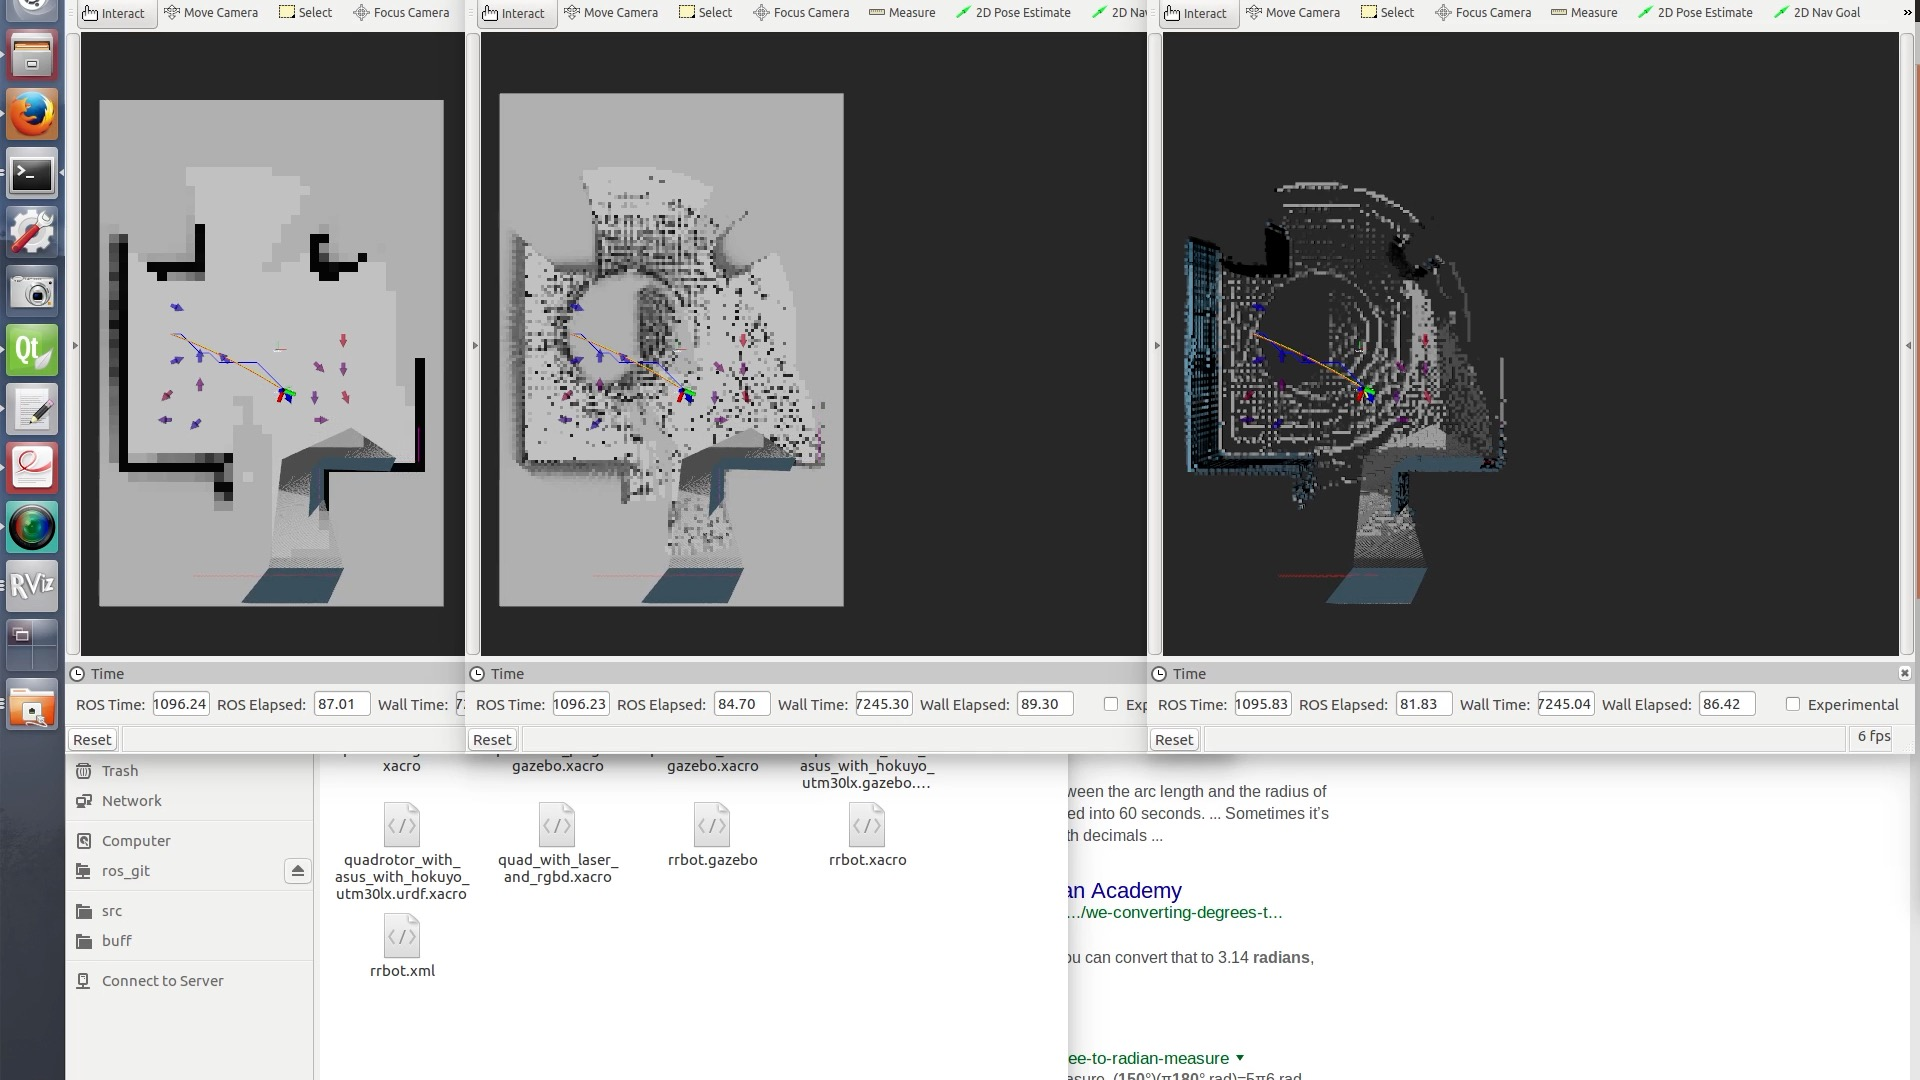
\includegraphics[trim = {41.5cm 17cm 14.3cm 3.8cm}, clip, height=\textwidth]{gazebo_1min.jpg}
        		\caption{$t=1$ min}
    	\end{subfigure}
    	\begin{subfigure}[t]{0.24\columnwidth}
           	\centering
          	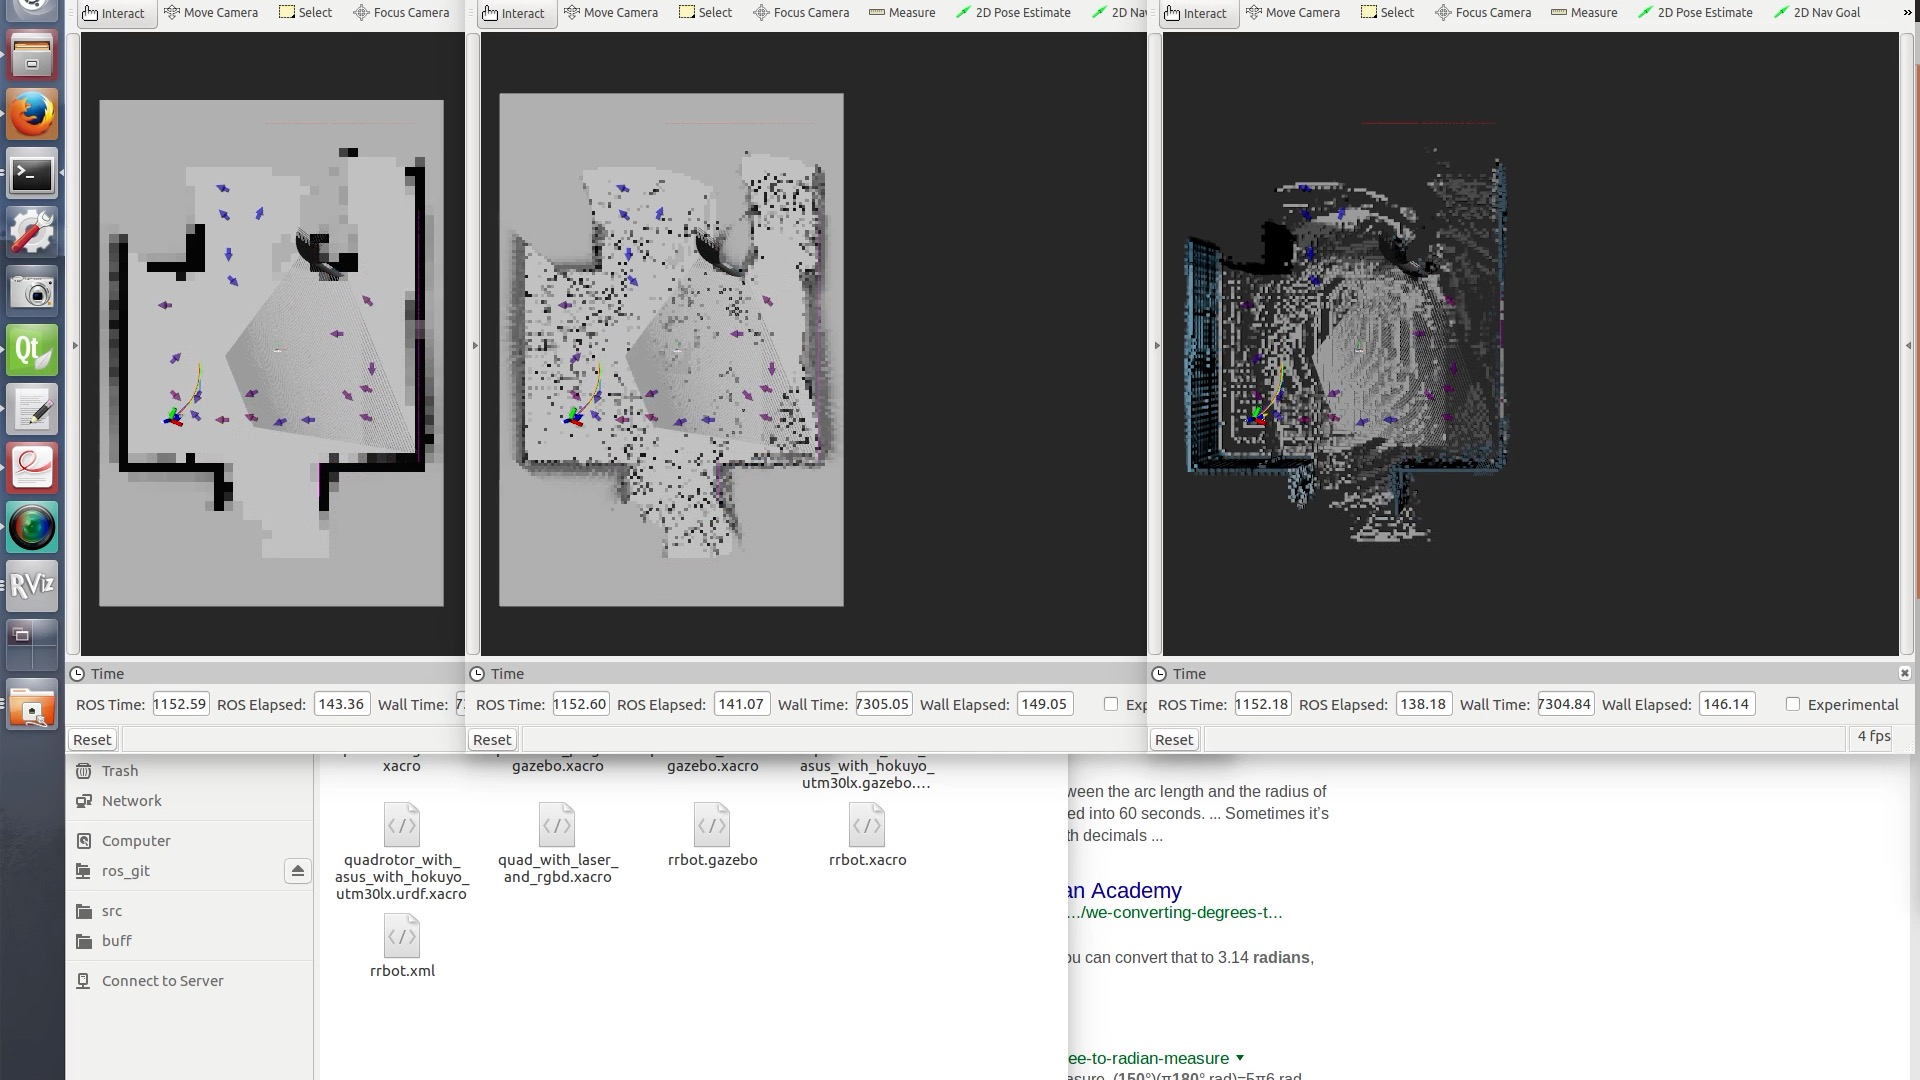
\includegraphics[trim = {41.5cm 17cm 14.3cm 3.8cm}, clip, height=\textwidth]{gazebo_2min.jpg}
        		\caption{$t=2$ min}
    	\end{subfigure}
    	\begin{subfigure}[t]{0.24\columnwidth}
           	\centering
          	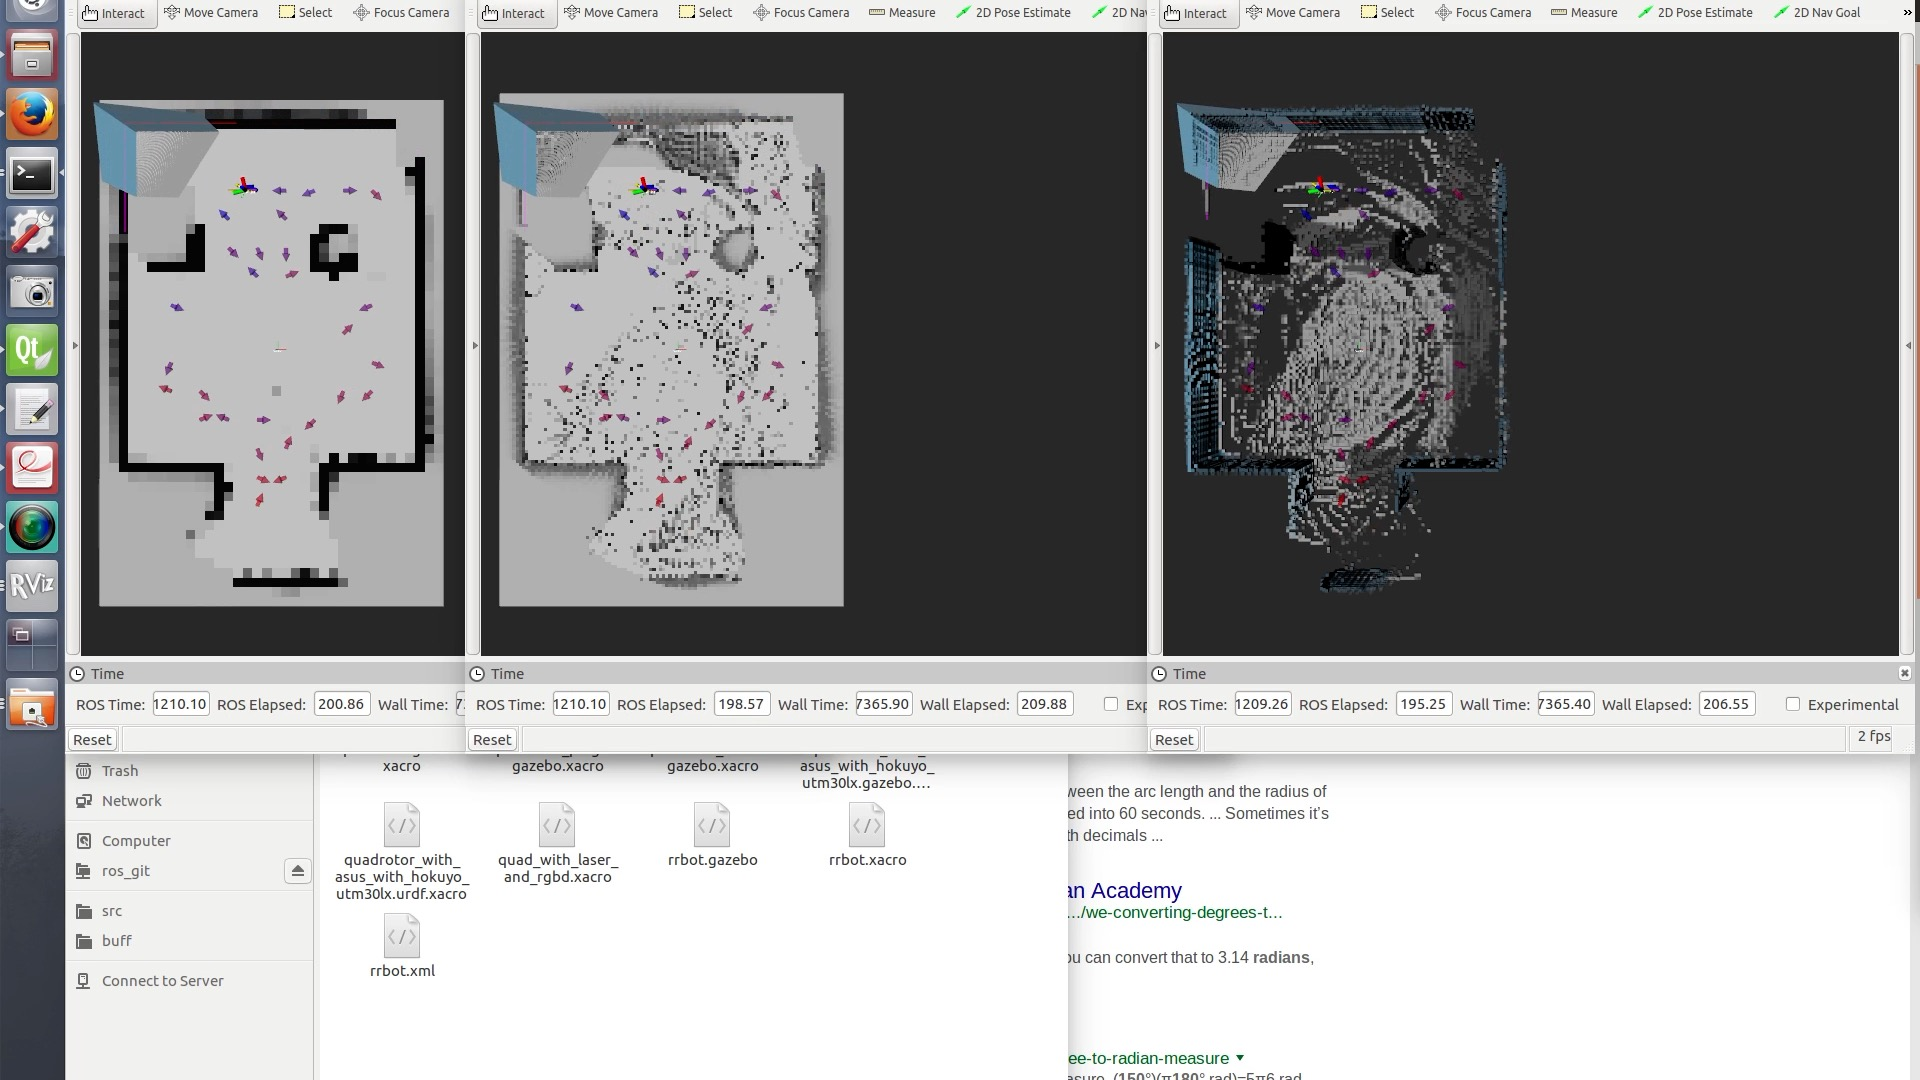
\includegraphics[trim = {41.5cm 17cm 14.3cm 3.8cm}, clip, height=\textwidth]{gazebo_3min.jpg}
        		\caption{$t=3$ min}
   	\end{subfigure}
    	\begin{subfigure}[t]{0.24\columnwidth}
           	\centering
          	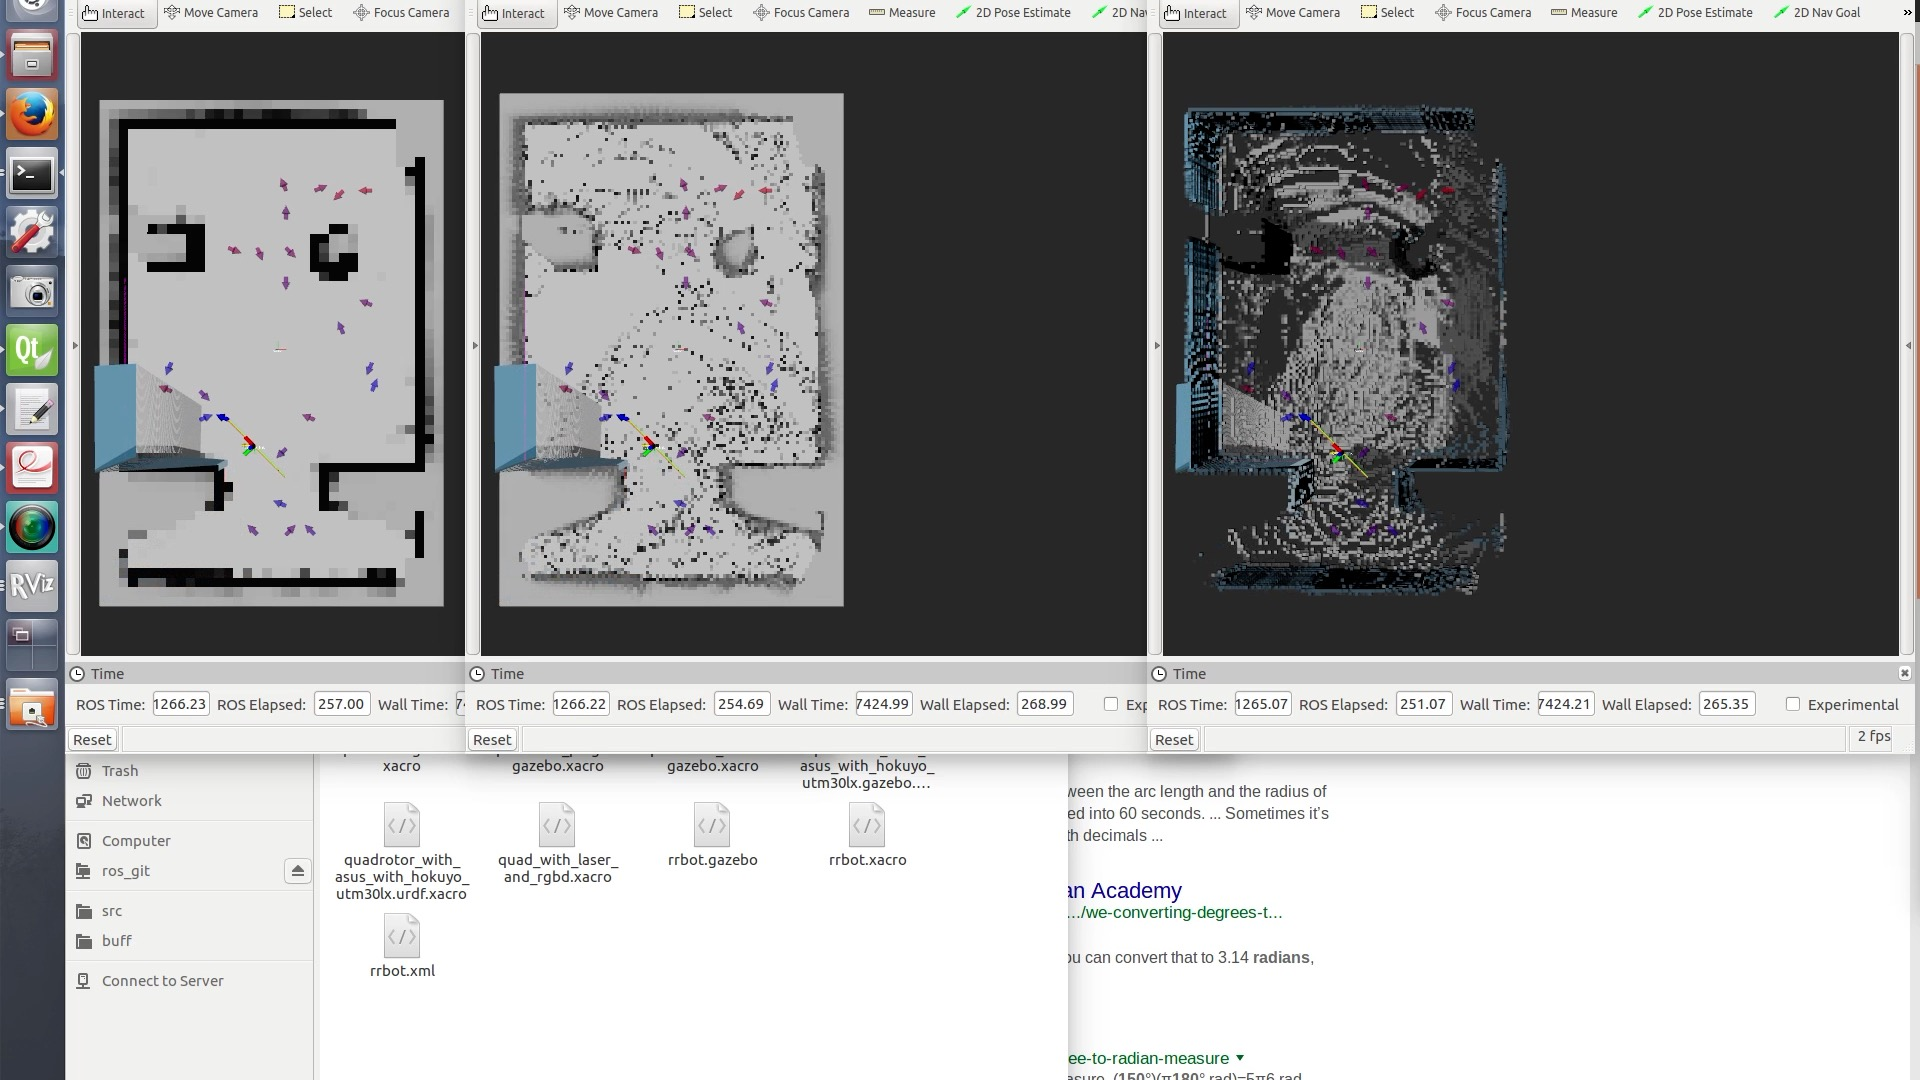
\includegraphics[trim = {41.5cm 17cm 14.3cm 3.8cm}, clip, height=\textwidth]{gazebo_4min.jpg}
        		\caption{$t=4$ min}
    	\end{subfigure}
	\begin{subfigure}[t]{0.24\columnwidth}
	\vspace*{0.15\columnwidth}
           	\centering
          	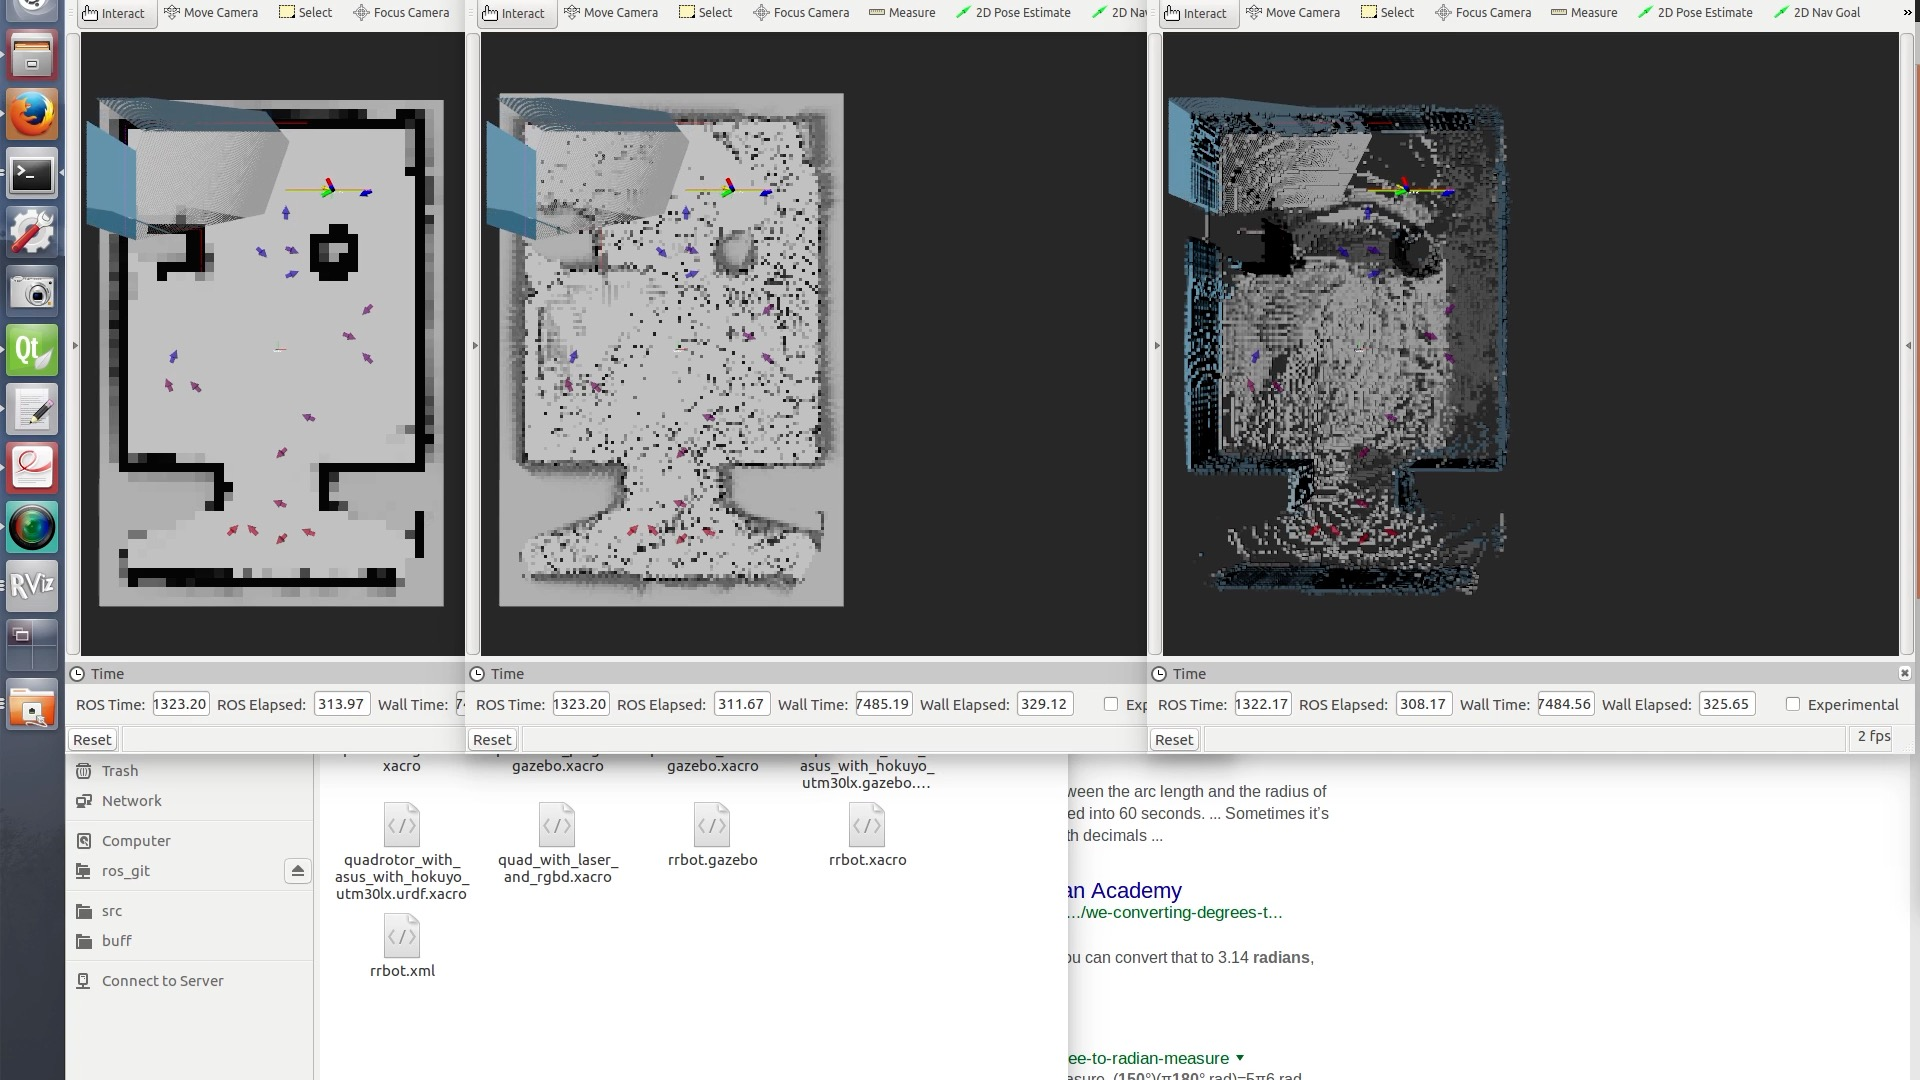
\includegraphics[trim = {41.5cm 17cm 14.3cm 3.8cm}, clip, height=\textwidth]{gazebo_5min.jpg}
        		\caption{$t=5$ min}
    	\end{subfigure}
    	\begin{subfigure}[t]{0.24\columnwidth}
	\vspace*{0.15\columnwidth}
           	\centering
          	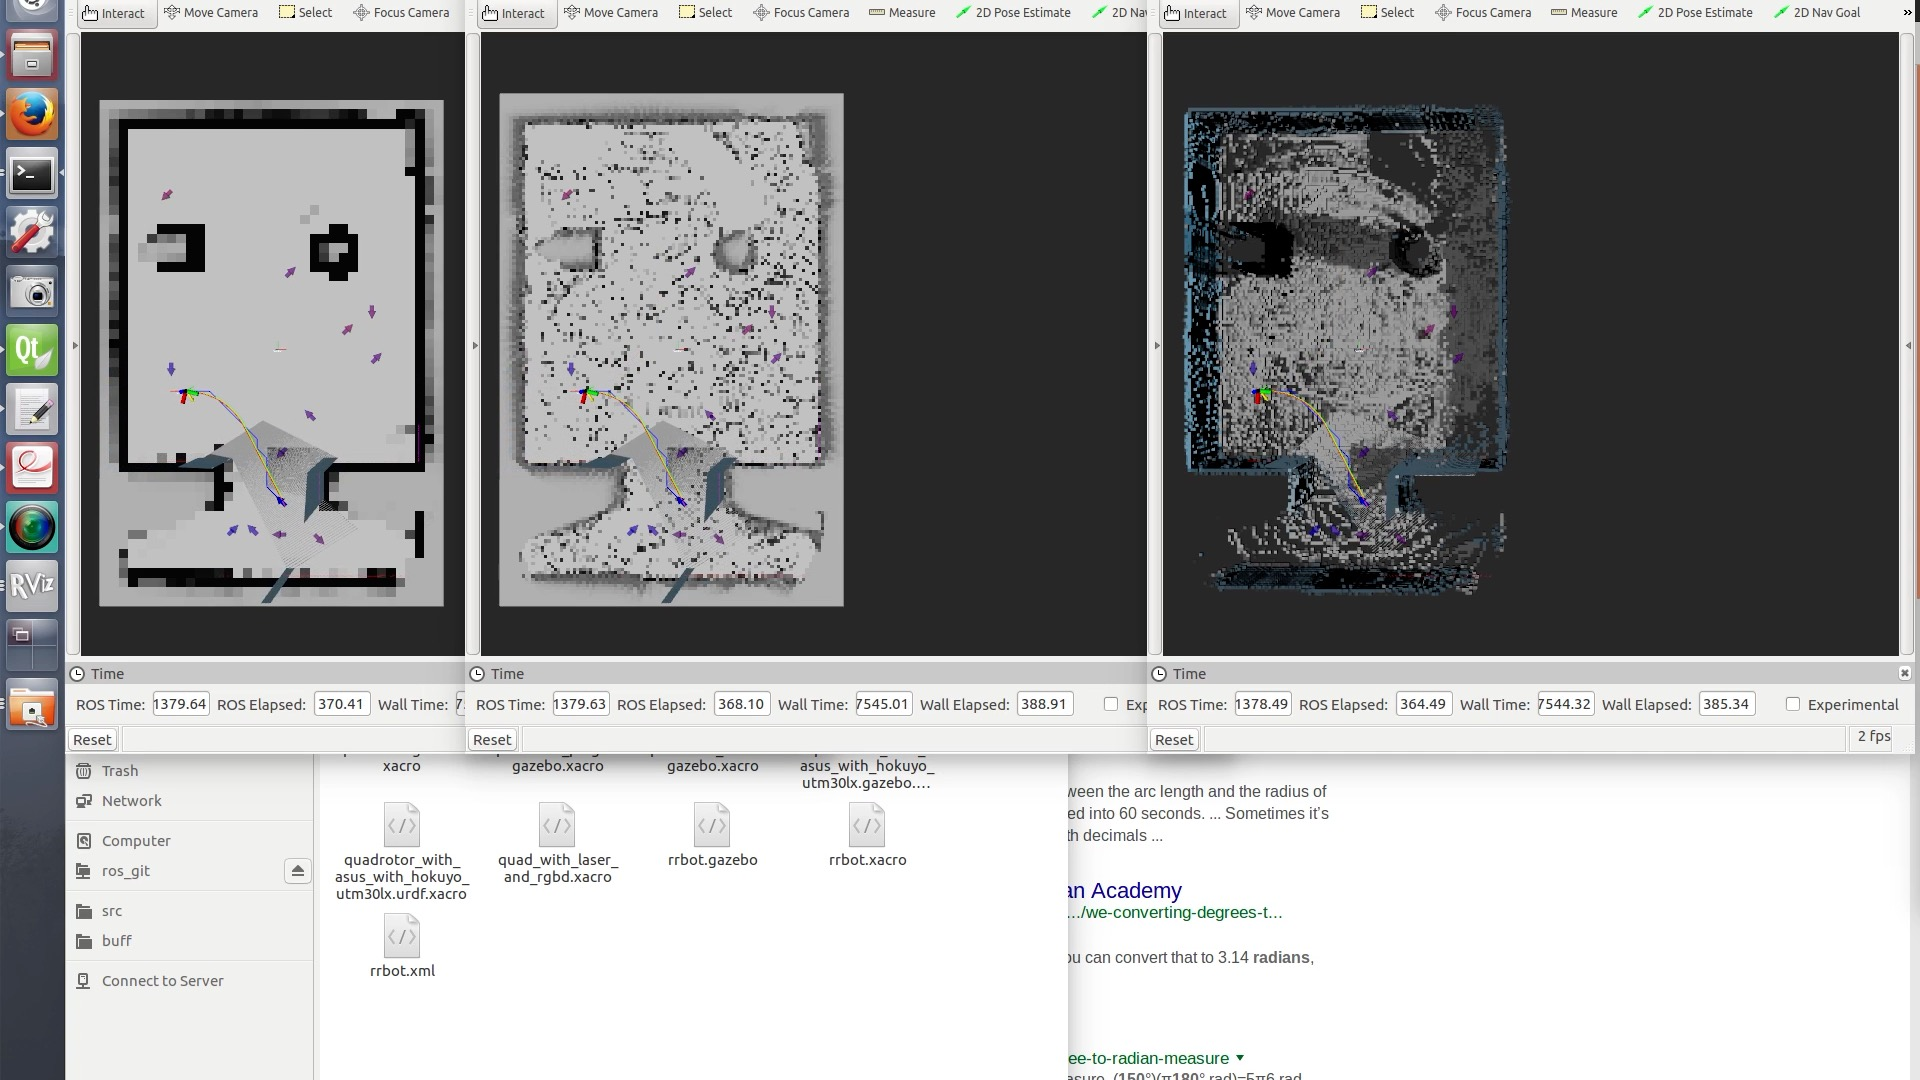
\includegraphics[trim = {41.5cm 17cm 14.3cm 3.8cm}, clip, height=\textwidth]{gazebo_6min.jpg}
        		\caption{$t=6$ min}
    	\end{subfigure}
    	\begin{subfigure}[t]{0.24\columnwidth}
	\vspace*{0.15\columnwidth}
           	\centering
          	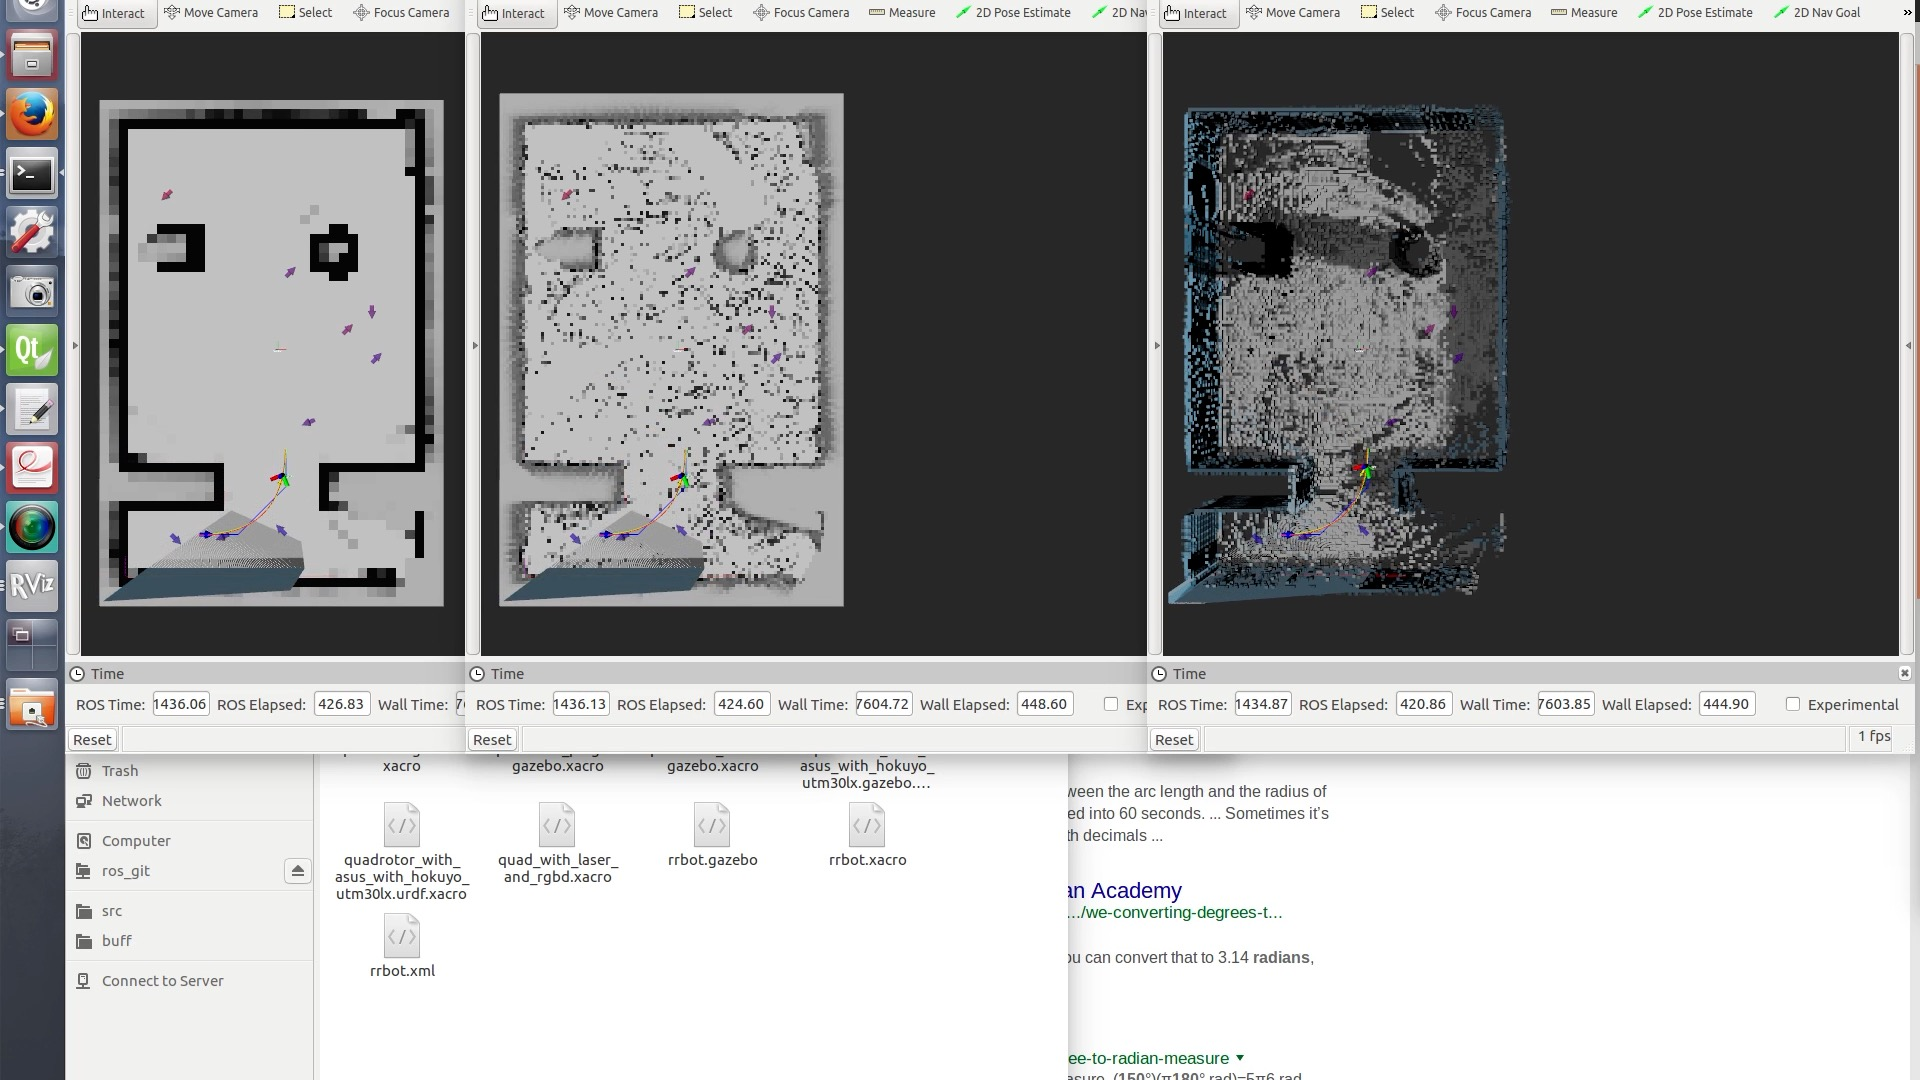
\includegraphics[trim = {41.5cm 17cm 14.3cm 3.8cm}, clip, height=\textwidth]{gazebo_7min.jpg}
        		\caption{$t=7$ min}
   	\end{subfigure}
    	\begin{subfigure}[t]{0.24\columnwidth}
	\vspace*{0.15\columnwidth}
           	\centering
          	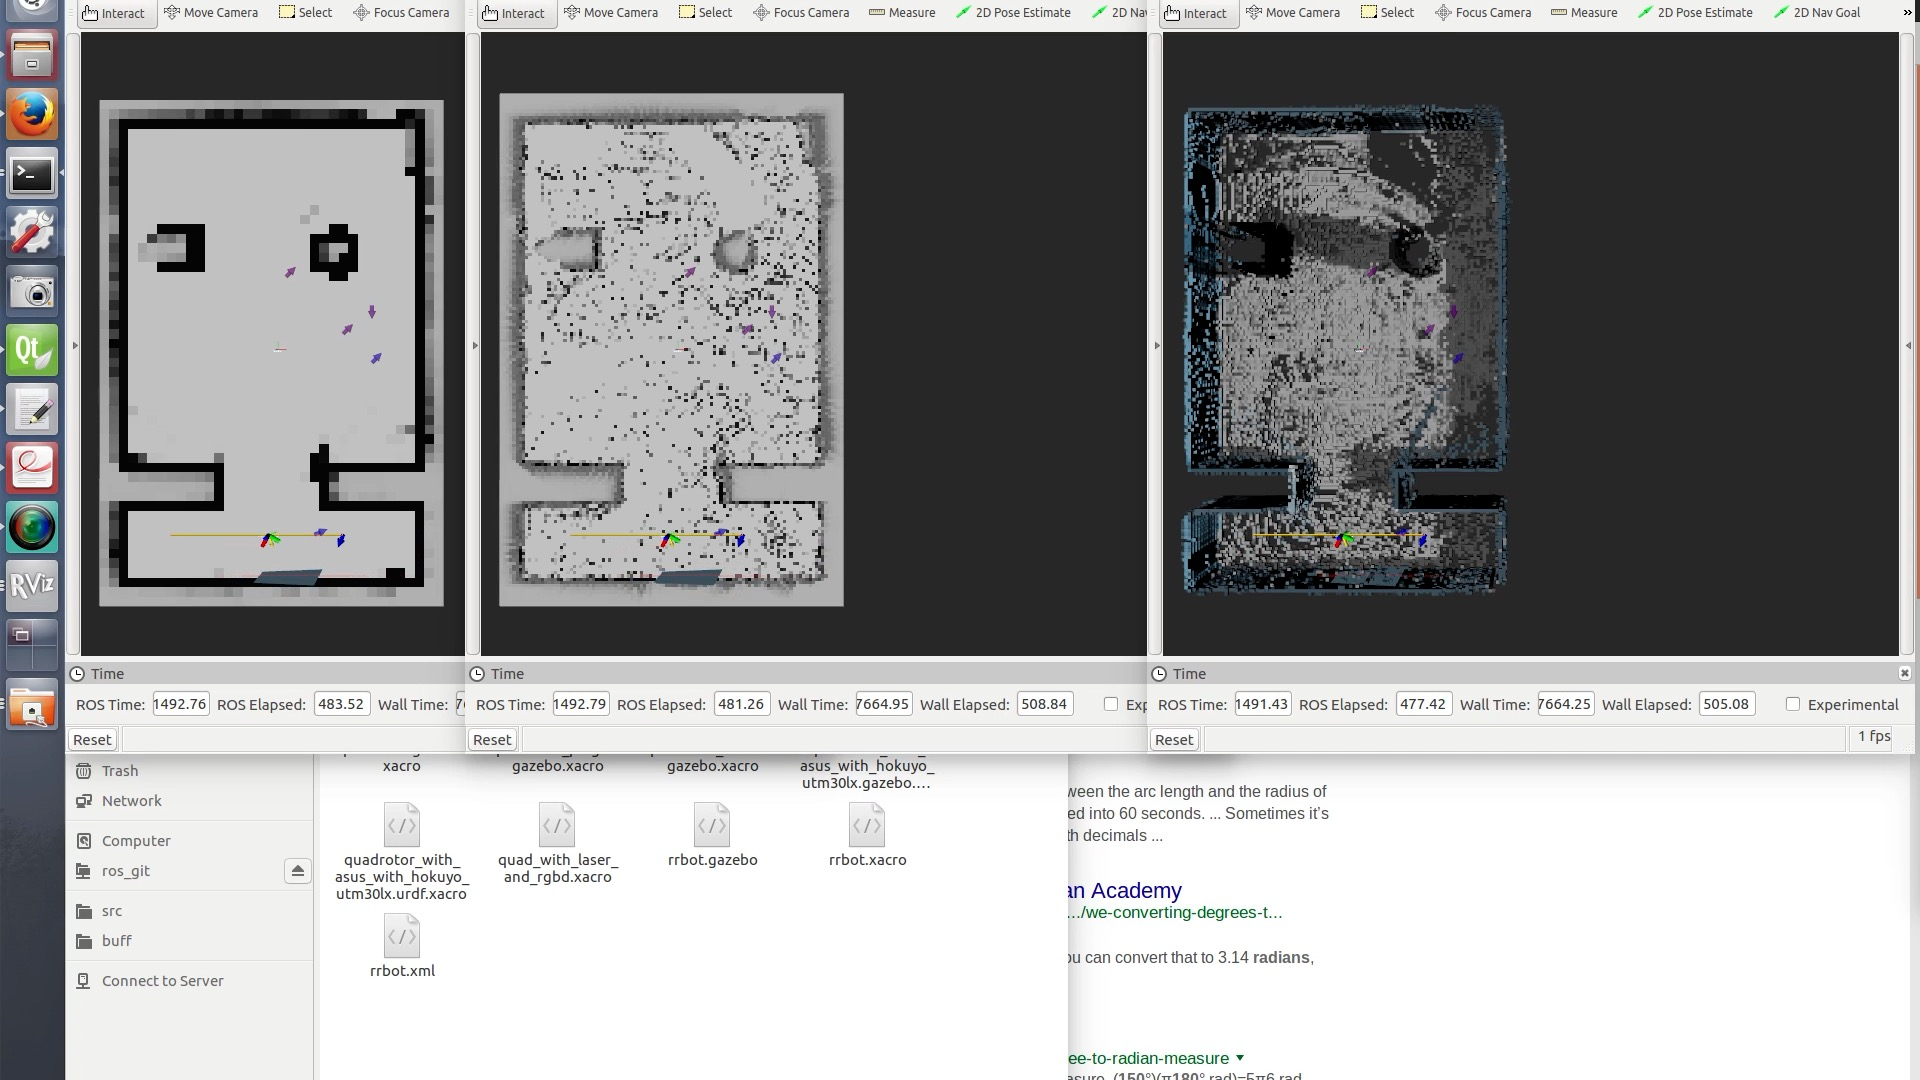
\includegraphics[trim = {41.5cm 17cm 14.3cm 3.8cm}, clip, height=\textwidth]{gazebo_8min.jpg}
        		\caption{$t=8$ min}
    	\end{subfigure}
%\includegraphics[width=2.5in]{myfigure}
% where an .eps filename suffix will be assumed under latex, 
% and a .pdf suffix will be assumed for pdflatex; or what has been declared
% via \DeclareGraphicsExtensions.
\caption{Simulated 3D Occupancy Grid Map}
\label{fig:sim3DMap}
\end{figure}


\begin{figure}
	\centering
	\begin{subfigure}[t]{0.3\columnwidth}
           	\centering
          	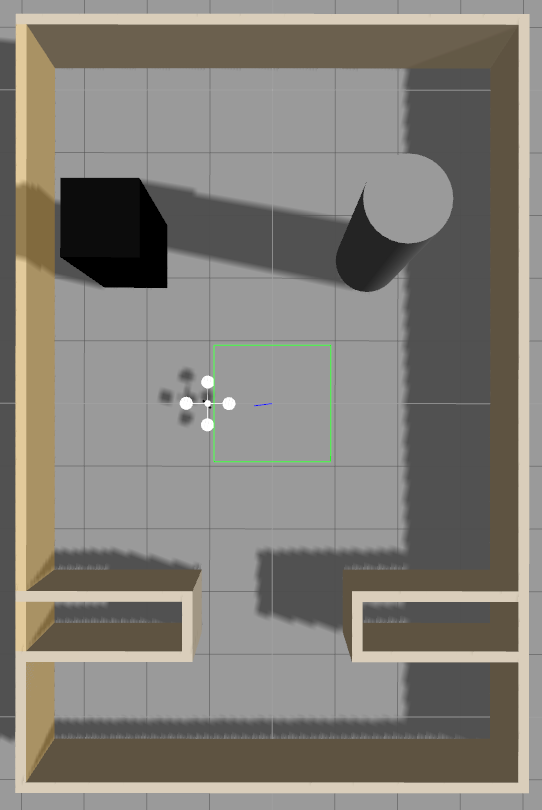
\includegraphics[height=1.5\textwidth]{gazebo_view.png}
        		\caption{Environment}
    	\end{subfigure}
		\hspace*{0.05cm}
    	\begin{subfigure}[t]{0.3\columnwidth}
           	\centering
          	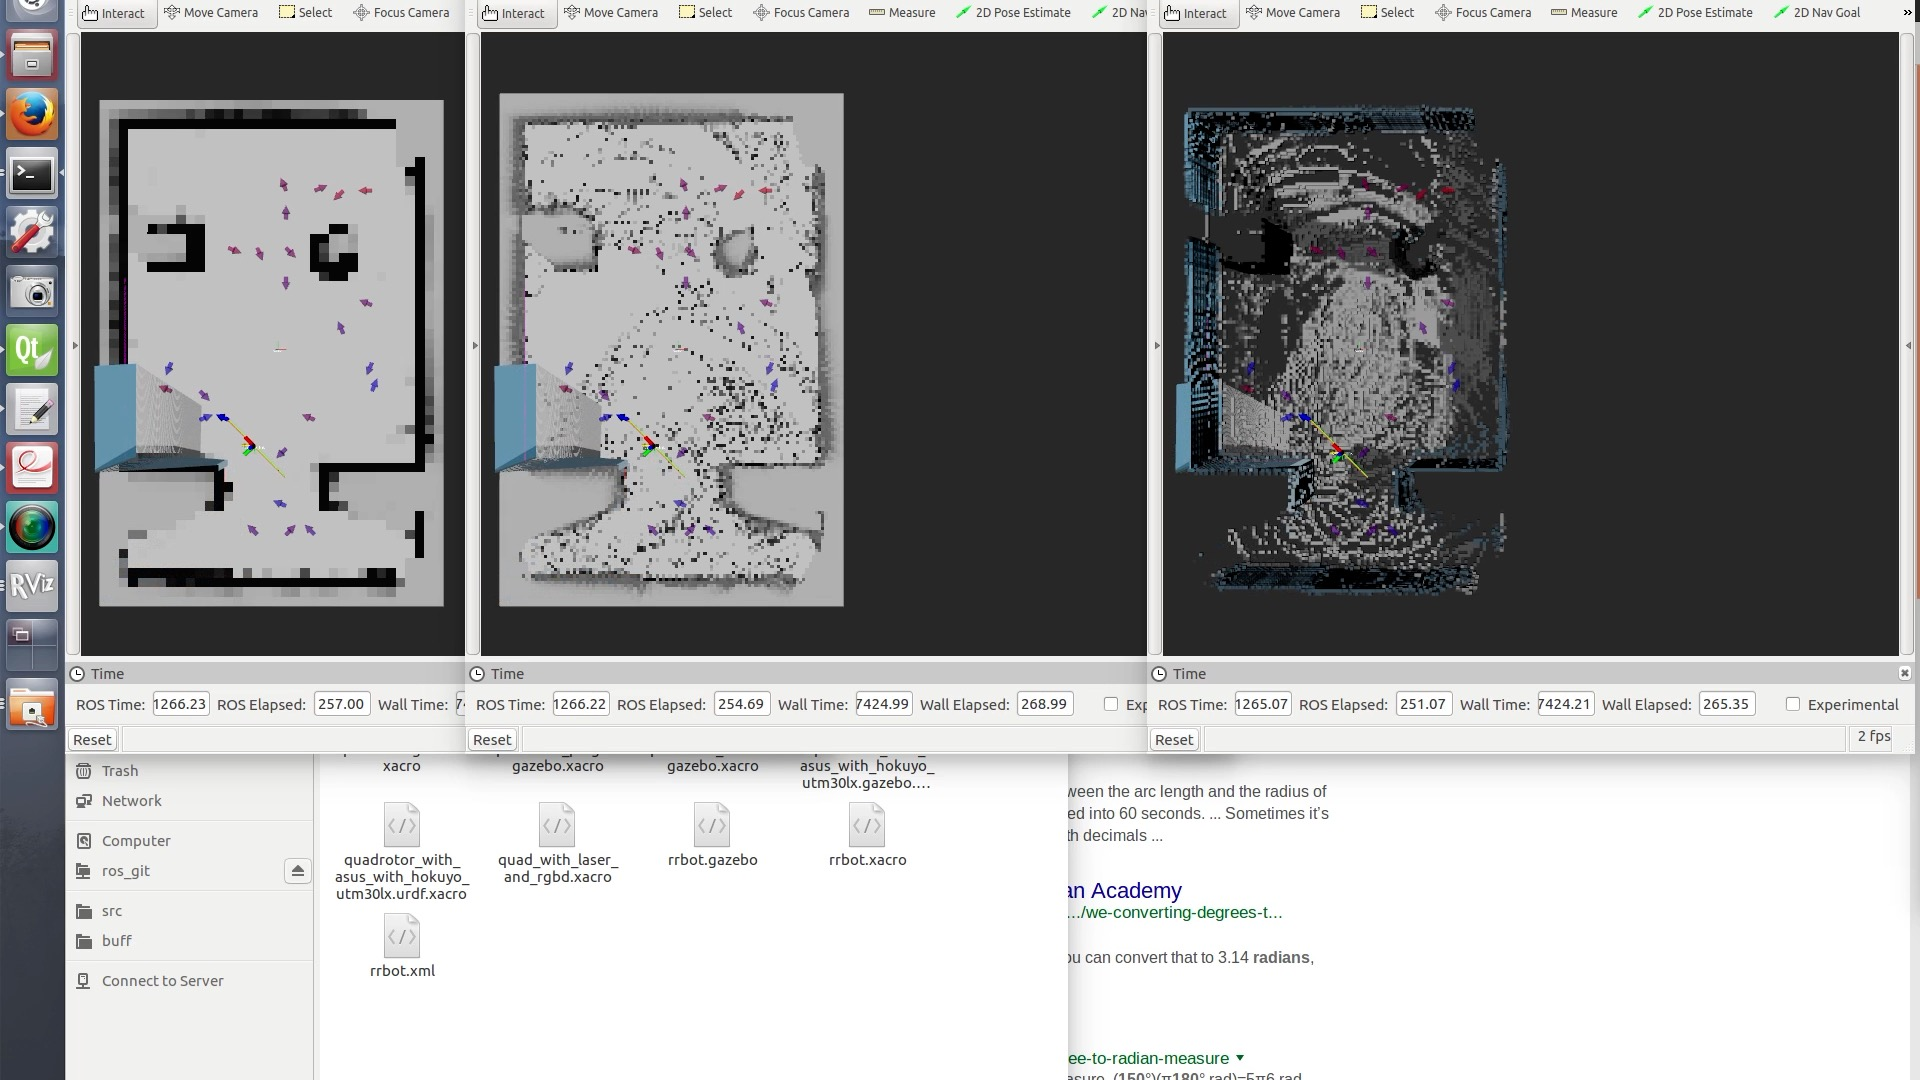
\includegraphics[trim = {3.6cm 17cm 52.5cm 4cm}, clip, height=1.5\textwidth]{gazebo_4min.jpg}
        		\caption{Collision Map}
    	\end{subfigure}
	\hspace*{0.1cm}
	\begin{subfigure}[t]{0.3\columnwidth}
           	\centering
          	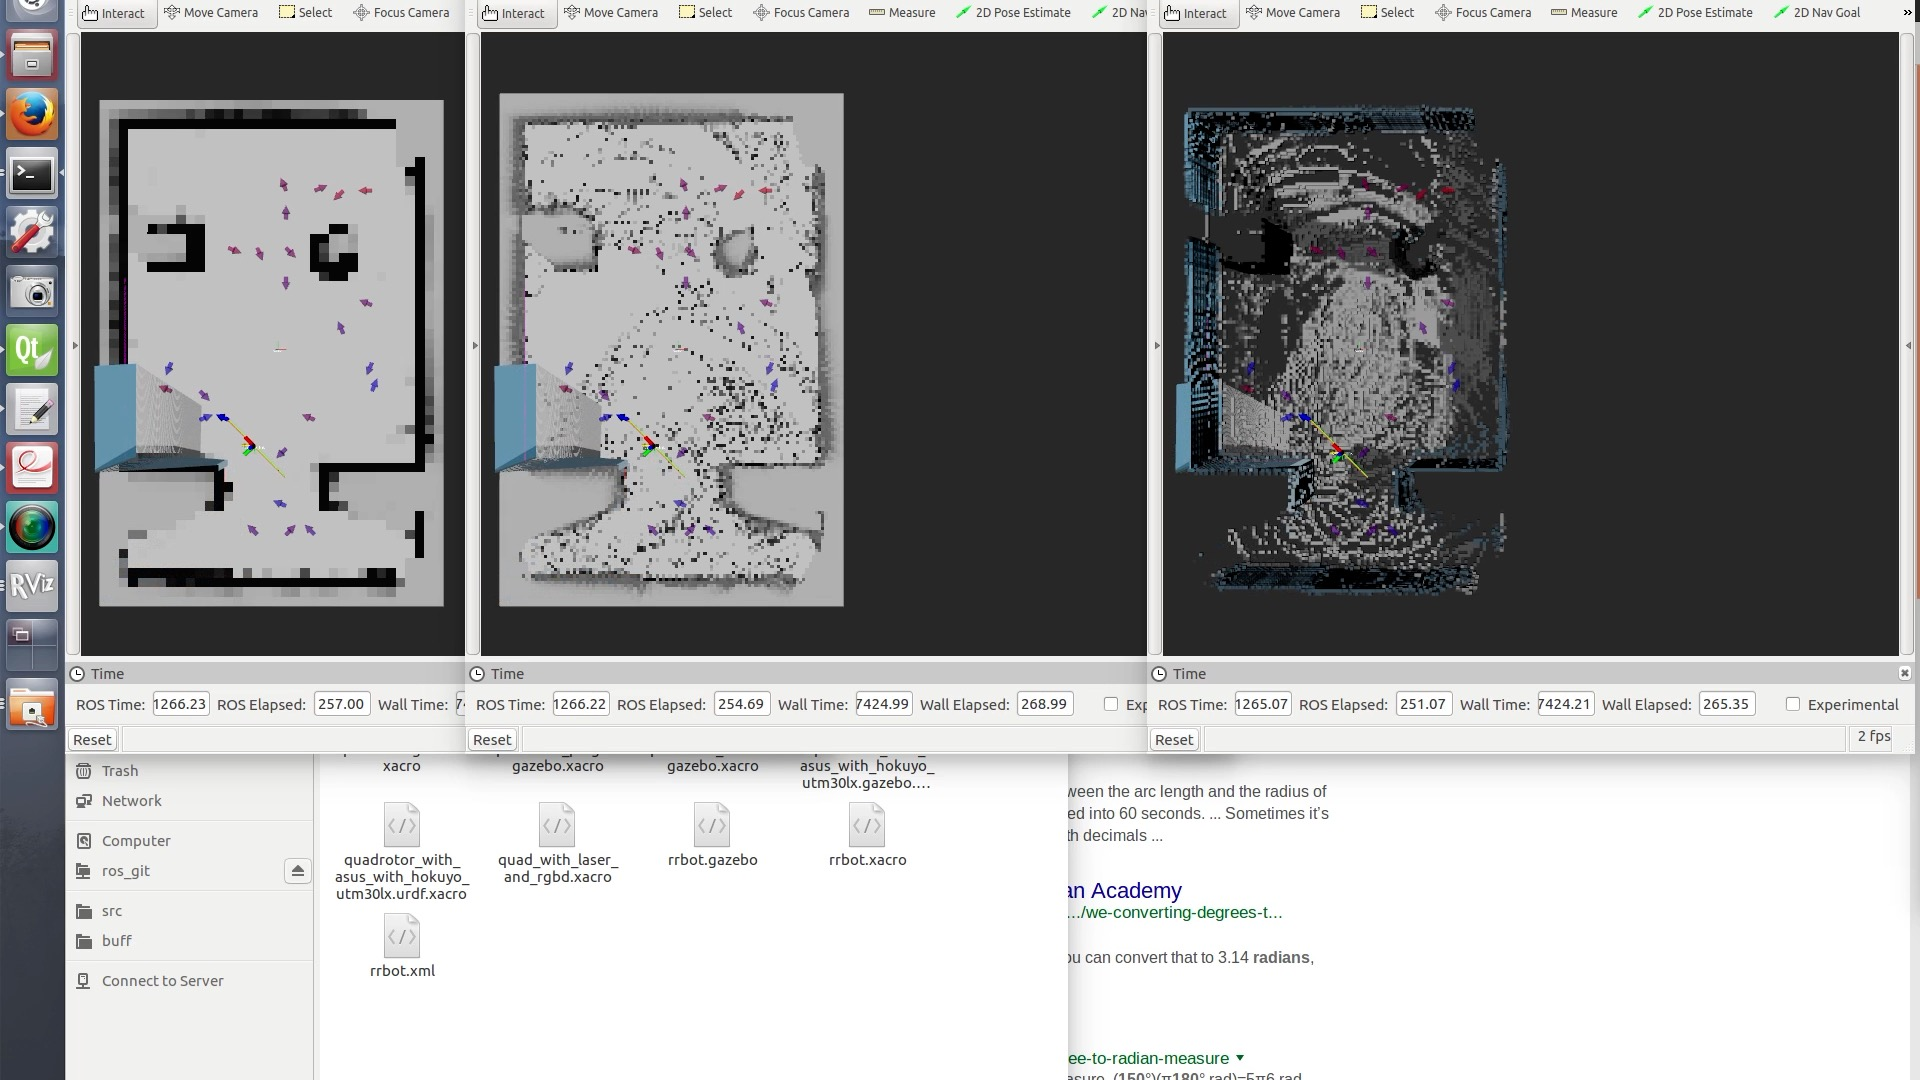
\includegraphics[trim = {18cm 17cm 38.1cm 4cm}, clip, height=1.5\textwidth]{gazebo_4min.jpg}
        		\caption{Entropy Map}
		\label{fig:sim2DmapsC}
    	\end{subfigure}
%\includegraphics[width=2.5in]{myfigure}
% where an .eps filename suffix will be assumed under latex, 
% and a .pdf suffix will be assumed for pdflatex; or what has been declared
% via \DeclareGraphicsExtensions.
\caption{Simulated Environment and 2D Projected Maps at $4$ min}
\label{fig:sim2Dmaps}
\end{figure}

\begin{figure}[!t]
	\centering
	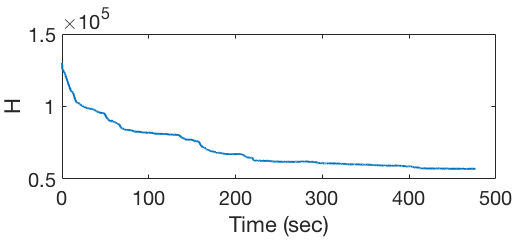
\includegraphics[width=0.9\textwidth]{entropy_gazebo_aspect3by1.png}
	\caption{Simulated Environment Map Entropy}
	\label{fig:simH}
\end{figure}

The two-map approach both exhibits advantages and disadvantages. The exploration algorithm successfully avoided collisions and gave way to a fairly complete 3D occupancy grid. The floor, which is not always visible, is properly estimated in most places. Conversely, this attention to detail has negative consequences that encourage the robot to repeatedly look at the same regions from different vantage points.
Since an entropy map cell is composed from many 3D grid cells single-stacked vertically, if just one of these 3D map cells is not captured or hardly captured, the entropy map cell will be recorded as quite uncertain, shown covering numerous locations in Figure~\ref{fig:sim2DmapsC}. The robot may attempt to measure this space again, even when other regions might more strongly warrant observation. These periods of sluggish entropy decrease are shown with flatter sections of Figure~\ref{fig:simH}. In short, this algorithm successfully explores the space collision-free while producing a complete map, but over-attention to just a few uncertain cells has negative consequences on the exploration speed.






% TODO: move below to experimental results
%\section{Exploring a Large Room}
% IRC18 result: Figure 4, 5, 6, 7


\section{Conclusions}

In this chapter, we proposed an extension of exact probabilistic occupancy grid mapping from 2D to 3D, then proposed a simplified autonomous exploration scheme for vertically-uniform environments. Two versions of the projected map, namely one for collision and one for entropy, are used in a numerical example. The collision and entropy combination map is applied to an experimental result in Chapter \ref{chap:Experiments}.



